% Optical Fiber Polarization Controller
% Author: Jimi Oke
\documentclass{article}
\usepackage{tikz}
\begin{document}
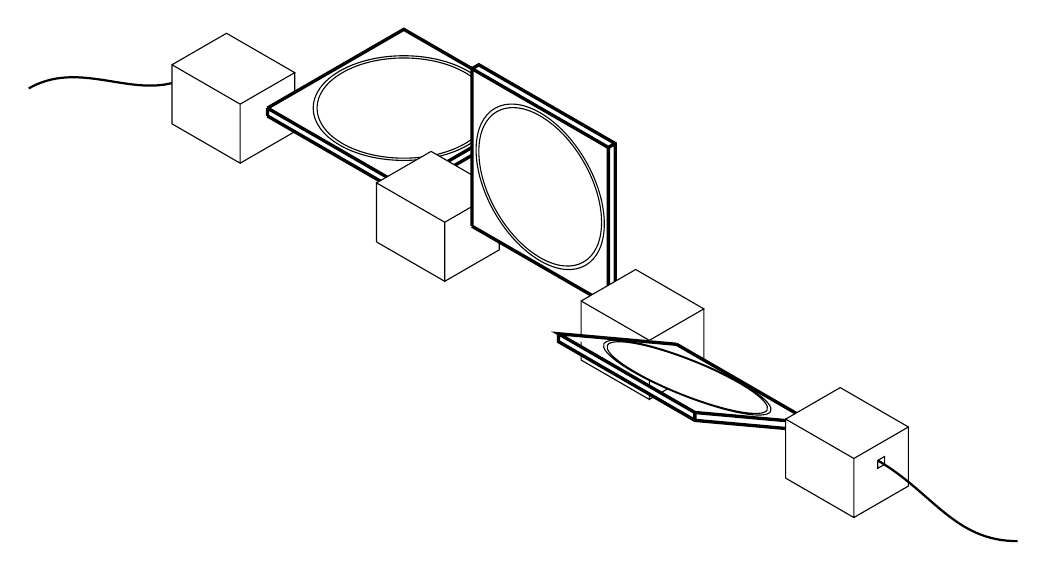
\begin{tikzpicture}[x={(0.866cm,-0.5cm)},
  y={(0.866cm,0.5cm)}, z={(0cm,1cm)}]
\tikzstyle{paddle}=[very thick, fill=white]
\coordinate (O) at (0, 0, 0);

% fiber in
\draw[thick] (0,-1.5,0) to[out=30,in=220] (1,0,0);

% first divider
\draw[fill=white] (1,-.4,-.5) -- (2,-.4,-.5) -- (2,-.4,.25) --
      (1,-.4,.25) -- (1,-.4,-.5)
      (2,-.4,.25) -- (2,.4,.25) -- (1,.4,.25) -- (1,-.4,.25)
      (2,.4,.25) -- (2,.4,-.5) -- (2,-.4,-.5);

% first paddle
\draw[paddle] 
      (2,0,0) -- (4,0,0) -- (4,2,0) -- (2,2,0) -- (2,0,0) % first face
      (2,0,0) -- (2,0,-.1)
      (4,0,0) -- (4,0,-.1)
      (2,0,-.1) -- (4,0,-.1) -- (4,2,-.1);
\draw (3,1,0) circle (.94)
      (3,1,0) circle (.9);

% second divider
\draw[fill=white] (4,-.4,-.5) -- (5,-.4,-.5) -- (5,-.4,.25) -- 
      (4,-.4,.25) -- (4,-.4,-.5)
      (5,-.4,.25) -- (5,.4,.25) -- (4,.4,.25) -- (4,-.4,.25)
      (5,.4,.25) -- (5,.4,-.5) -- (5,-.4,-.5);

% second paddle
\filldraw[paddle]
     (5,0,0) -- (7,0,0) -- (7,0,2) -- (5,0,2) -- (5,0,0) % first face
     (7,0,0) -- (7,.1,0) -- (7,.1,2) -- (5,.1,2) -- (5,0,2)
     (7,.1,2) -- (7,0,2);

% third divider
\draw[fill=white] (7,-.4,-.5) -- (8,-.4,-.5) -- (8,-.4,.25) --
      (7,-.4,.25) -- (7,-.4,-.5)
      (8,-.4,.25) -- (8,.4,.25) -- (7,.4,.25) -- (7,-.4,.25)
      (8,.4,.25) -- (8,.4,-.5) -- (8,-.4,-.5);

% third paddle
\filldraw[paddle] 
     (8,0,0) -- (10,0,0) -- (10, -1.732,1) -- (8,-1.732,1)
     -- (8,0,0)
(8,-1.732,1) -- (8,-1.732,.9) -- (10,-1.732,.9) -- (10,0,-.1)
-- (10,0,0)
(10,-1.732,.9) -- (10,-1.732,1);

% fourth divider  
\draw[fill=white] (10,-.4,-.5) -- (11,-.4,-.5) -- (11,-.4,.25) --
      (10,-.4,.25) -- (10,-.4,-.5)
      (11,-.4,.25) -- (11,.4,.25) -- (10,.4,.25) -- (10,-.4,.25)
      (11,.4,.25) -- (11,.4,-.5) -- (11,-.4,-.5);

\begin{scope}[x={(0.866cm,-0.5cm)},y={(0,1cm)}]
\draw (6,0,1) circle (.94)
      (6,0,1) circle (.9);
\end{scope}

\begin{scope}[x={(0.866cm,-0.5cm)},y={(-.73cm,.077cm)}]
\draw[fill=white] (9,1) circle (.94)
      (9,1) circle (.9);
\end{scope}

% fiber exit
\draw (11,-.05,.05) -- (11,.05,.05) --
     (11,.05,-.05) -- (11,-.05,-.05) -- (11,-.05,.05);
\draw[thick] (10.95,0,0) to[out=-30,in=180] (12,1,-1);
\end{tikzpicture}
\end{document} 